% !TEX encoding = UTF-8 Unicode
%%%%%%%%%%%%%%%%%%%%%%%%%%%%%%%%%%%%%%%%%
% Beamer Presentation
% LaTeX Template
% Version 1.0 (10/11/12)
%
% This template has been downloaded from:
% http://www.LaTeXTemplates.com
%
% License:
% CC BY-NC-SA 3.0 (http://creativecommons.org/licenses/by-nc-sa/3.0/)
%
%%%%%%%%%%%%%%%%%%%%%%%%%%%%%%%%%%%%%%%%%

%----------------------------------------------------------------------------------------
%	PACKAGES AND THEMES
%----------------------------------------------------------------------------------------
\documentclass[french]{beamer}
\usepackage{beamerthemesplit}
\usepackage[utf8]{inputenc}
\usepackage[T1]{fontenc}
\usepackage{anyfontsize}
\usepackage{amsmath,amssymb,amsfonts,amsbsy}
\usepackage{eqnarray,amsmath}
\usepackage{booktabs}
\usepackage{subfig}
\usepackage{multirow}
\usepackage{booktabs}
\usepackage{dcolumn}
% algorithms
\usepackage{algorithmic}
\usepackage{algorithm}
% mathematical
\usepackage{amssymb}
\usepackage{pifont}
\usepackage{graphicx}
\usepackage{epstopdf}
\usepackage{animate}
\usepackage{hyperref}

\graphicspath{{fig}}

\epstopdfDeclareGraphicsRule{.gif}{png}{.png}{convert gif:#1 png:\OutputFile}
\AppendGraphicsExtensions{.gif}% http://ctan.org/pkg/pifont
\definecolor{MediumSeaGreen}{rgb}{0.2344,0.6992,0.4414}
\newcommand{\cmark}{\textcolor{MediumSeaGreen}{\ding{52}}}%
\newcommand{\xmark}{\textcolor{red}{\ding{54}}}%
\renewcommand{\multirowsetup}{\centering}		% to use centering in multirow command	%DB
\newcommand{\B}[1]{\textbf{#1}}	% to obtain bold fonts %DB
\newcommand{\DB}[1]{\textcolor{red}{#1}}	% to makes a highlighted text in hcl color
\newcommand{\T}[1]{\textcolor{black}{#1}}	
\graphicspath{{fig/}}
\newcommand{\TOM}[1]{\textcolor{red}{[\textsc{TOM}: \emph{#1}]}}
\newcolumntype{C}[1]{>{\centering\arraybackslash}p{#1}} % to force centered columns with a specific width
%\newcolumntype{L}[1]{>{\raggedright\arraybackslash}p{#1}}
%\newcolumntype{R}[1]{>{\raggedleft\arraybackslash}p{#1}}
\renewcommand{\multirowsetup}{\centering}	% to use centering in multirow command	%DB
\def\s{\hphantom{0}}	% {\s} space corresponding to a number  (for tables centering) %DB
\def\x{\hphantom{$-$}}	% {\x} space corresponding to a negative (for tables centering) 
\newcommand{\tabitem}{~~\llap{\textbullet}~~}



\DeclareGraphicsExtensions{.pdf,.png,.eps,.jpg}
\tolerance=1000
\hyphenpenalty=1000
\overfullrule=1mm
\providecommand{\ve}[1]{{\pmb{#1}}} %
\providecommand{\mat}[1]{{\pmb{#1}}} %
\DeclareMathOperator{\Real}{\mathbb{R}}
\DeclareMathOperator{\Natural}{\mathbb{N}}
\mode<presentation>{

% The Beamer class comes with a number of default slide themes
% which change the colors and layouts of slides. Below this is a list
% of all the themes, uncomment each in turn to see what they look like.

% \usetheme{default}
% \usetheme{AnnArbor}
% \usetheme{Antibes}
%\usetheme{Bergen}
%\usetheme{Berkeley}
% % % % % \usetheme{Berlin}
%\usetheme{Boadilla}
%\usetheme{CambridgeUS}
%\usetheme{Copenhagen}
%\usetheme{Darmstadt}
%\usetheme{Dresden}
%\usetheme{Frankfurt}
%\usetheme{Goettingen}
%\usetheme{Hannover}
%\usetheme{Ilmenau}
%\usetheme{JuanLesPins}
%\usetheme{Luebeck}
\usetheme{Madrid}
%\usetheme{Malmoe}
%\usetheme{Marburg}
%\usetheme{Montpellier}
%\usetheme{PaloAlto}
%\usetheme{Pittsburgh}
%\usetheme{Rochester}
%\usetheme{Singapore}
% \usetheme{Szeged}
%\usetheme{Warsaw}

% As well as themes, the Beamer class has a number of color themes
% for any slide theme. Uncomment each of these in turn to see how it
% changes the colors of your current slide theme.

%\usecolortheme{albatross}
%\usecolortheme{beaver}
%\usecolortheme{beetle}
%\usecolortheme{crane}
%\usecolortheme{dolphin}
%\usecolortheme{dove}
%\usecolortheme{fly}
%\usecolortheme{lily}
%\usecolortheme{orchid}
%\usecolortheme{rose}
%\usecolortheme{seagull}
\usecolortheme{seahorse}
%\usecolortheme{whale}
%\usecolortheme{wolverine}

%\setbeamertemplate{footline} % To remove the footer line in all slides uncomment this line
%\setbeamertemplate{footline}[page number] % To replace the footer line in all slides with a simple slide count uncomment this line

%\setbeamertemplate{navigation symbols}{} % To remove the navigation symbols from the bottom of all slides uncomment this line
}

\usepackage{graphicx} % Allows including images
\usepackage{booktabs} % Allows the use of \toprule, \midrule and \bottomrule in tables

% \usepackage[font=Times,timeinterval=30,timeduration=15,timewarningfirst=80,timewarningsecond=90,colorwarningfirst=blue,fillcolorwarningfirst=white!60!yellow, fillcolorwarningsecond=white!10!yellow, resetatpages=2]{tdclock}


% \addtobeamertemplate{navigation symbols}{}{%
%     \usebeamerfont{footline}%
%     \usebeamercolor[fg]{footline}%
%     \hspace{1em}%
%     \insertframenumber/\inserttotalframenumber
% }

%----------------------------------------------------------------------------------------
%	TITLE PAGE
%----------------------------------------------------------------------------------------

\title[Recharge intelligente de VE]{Une approche d'apprentissage automatique pour la recharge intelligente des véhicules électriques} 
% \title[Recharge intelligente de VE \hspace{5mm} \cronominutes:\cronoseconds]{Une approche d'apprentissage automatique pour la recharge intelligente des véhicules électriques} 

\author[Karol Lina L\'opez]{\texorpdfstring{Karol Lina L\'opez\newline\href{mailto:karol-lina.lopez.1@ulaval.ca}{karol-lina.lopez.1@ulaval.ca}}{Karol Lina L\'opez}}
  \centering
 \titlegraphic{
 \begin{minipage}{0.33\textwidth}
 
\includegraphics[width=2.5cm]{REPARTI.jpg}
 \end{minipage}\hfill%
 \begin{minipage}{0.33\textwidth}
 
\includegraphics[width=2.5cm]{ul_logo.pdf}
 \end{minipage}\hfill%
 \begin{minipage}{0.33\textwidth}
 
\includegraphics[width=2.5cm]{LVSN2.png}
 \end{minipage}
}
\date{22 jan 2019} % Date, can be changed to a custom date


\begin{document}


{\setbeamercolor{block body}{bg=white}
\newcommand{\abs}[1]{\left\vert#1\right\vert}
\newcommand{\argmin}{\operatornamewithlimits{argmin}}
\newcommand{\argmax}{\operatornamewithlimits{argmax}}
\newcommand{\mean}{\operatornamewithlimits{mean}}

\begin{frame}
% \initclock
\titlepage % Print the title page as the first slide
\end{frame}
% 
% \begin{frame}
% \frametitle{Plan de la présentation} % Table of contents slide, comment this block out to remove it
% \fontsize{10}{1}{
% \tableofcontents[hideallsubsections]}% Throughout your presentation, if you choose to use \section{} and \subsection{} commands, these will automatically be printed on this slide as an overview of your presentation
% \end{frame}

% 
% 
% \begin{frame}
% \frametitle{}
% 
% \end{frame}

%----------------------------------------------------------------------------------------
%	PRESENTATION SLIDES
%----------------------------------------------------------------------------------------
%------------------------------------------------
%\section{Pourquoi des ensembles ?}

\section{Introduction}
\subsection{Contexte}

% \begin{frame}
% \frametitle{Prévision de l'achat de VEs}
% \begin{center}
% %\includegraphics<1>[width=0.7\linewidth]{Electric-Cars_sales.png}
% \includegraphics[width=0.7\linewidth]{BNEFforetast.jpg}
% %\includegraphics<2>[width=0.7\linewidth]{PEV-Sales-Canada.jpg}
% %\includegraphics<2>[width=0.7\linewidth]{previsiondemande.jpg}
% \end{center}
% \end{frame}
% 
% \begin{frame}
% \frametitle{Progression des ventes de Véhicules Électriques (VE)}
% \begin{center}
% %\includegraphics<1>[width=0.7\linewidth]{Electric-Cars_sales.png}
% % \includegraphics[width=0.8\linewidth]{salesEV.pdf}\\
% \includegraphics[width=0.8\linewidth]{fig/salesEV.pdf}\\
% \tiny{Source: Cobb, Jeff. 2017. "Top 10 Plug-in Vehicle Adopting Countries of 2016". HybridCars.com. Retrieved 2017-01-23.}
% %\includegraphics<2>[width=0.7\linewidth]{PEV-Sales-Canada.jpg}
% %\includegraphics<2>[width=0.7\linewidth]{previsiondemande.jpg}
% \end{center}
% \end{frame}


\begin{frame}
\frametitle{Véhicules électriques : portrait de la situation}
\vspace{-1.5em}
\begin{center}
\begin{figure}
\includegraphics<1>[width=0.9\linewidth]{evolution_ventes_ve.jpg}
\caption*{\only<1>{\tiny{Source: Bloomberg, 2017}}}

\includegraphics<2>[width=0.55\linewidth]{engagements.png}
\caption*{\only<2>{\tiny{Source: Radio-Canada, 2018}}}
\end{figure}
% \tiny{Source: Inauguration of the European Interoperability Centre for Electric Vehicles and Smart Grids}
% \tiny{Source: Report on the Economic and Environmental Impacts of Large-Scale Introduction on EV/PHEV. Shakoor and Aunedi, 2011}
\end{center}
\end{frame}

\begin{frame}
\frametitle{Intégrer les véhicules électriques dans le réseau électrique}
\begin{center}
\begin{figure}
\includegraphics<1>[width=0.9\linewidth]{smartgrid.png}
\caption*{\only<1>{\tiny{Source: Inauguration of the European Interoperability Centre for Electric Vehicles and Smart Grids}}}

\includegraphics<2>[width=0.6\linewidth]{picos.pdf}
\caption*{\only<2>{\tiny{Source: Report on the Economic and Environmental Impacts of Large-Scale Introduction on EV/PHEV. Shakoor $\&$ Aunedi, 2011}}}
\end{figure}
% \tiny{Source: Inauguration of the European Interoperability Centre for Electric Vehicles and Smart Grids}
% \tiny{Source: Report on the Economic and Environmental Impacts of Large-Scale Introduction on EV/PHEV. Shakoor and Aunedi, 2011}
\end{center}
\end{frame}

% 
% 
% 
% 
\begin{frame}
% %  http://www.intechopen.com/books/electric-vehicles-the-benefits-and-barriers/integration-of-electric-vehicles-in-the-electric-utility-systems
\frametitle{Stratégies pour la gestion de la demande}

\begin{tabular}{l|cc}
 			& \textbf{Orienté grille} & \textbf{Orienté utilisateur} \\ \hline
\emph{Objectifs} 	& 
\begin{minipage}{0.38\linewidth}\vspace{1em}
	\begin{itemize}
		\item Réduire la demande pic en puissance
		\item Réduire les coûts de production
	\end{itemize}\vspace{1em}
\end{minipage} 
& \begin{minipage}{0.38\linewidth}\vspace{1em}
	\begin{itemize}
		\item Assurer la disponibilité du véhicule
		\item Réduire le coût d'opération
	\end{itemize}\vspace{1em}
\end{minipage}  \\ \hline
\emph{Requis} & 
\begin{minipage}{0.38\linewidth}\vspace{1em}
	\begin{itemize}
		\item Données de consommation globales
		\item Infrastructure de communication complexe
	\end{itemize}
\end{minipage} 
& \begin{minipage}{0.38\linewidth}\vspace{1em}
	\begin{itemize}
		\item Données spécifiques à l'utilisateur
		\item Infrastructure de communication minimale
	\end{itemize}
\end{minipage}  \\
\end{tabular}
%
%\begin{columns}
%\begin{column}{0.5\linewidth}
%\begin{center}
%\textbf{Orienté grille}
%\end{center}
%\end{column}
%\begin{column}{0.5\linewidth}
%\begin{center}
%\textbf{Orienté utilisateur}
%\end{center}
%\end{column}
%\end{columns}

% \begin{center}
%\begin{figure}
%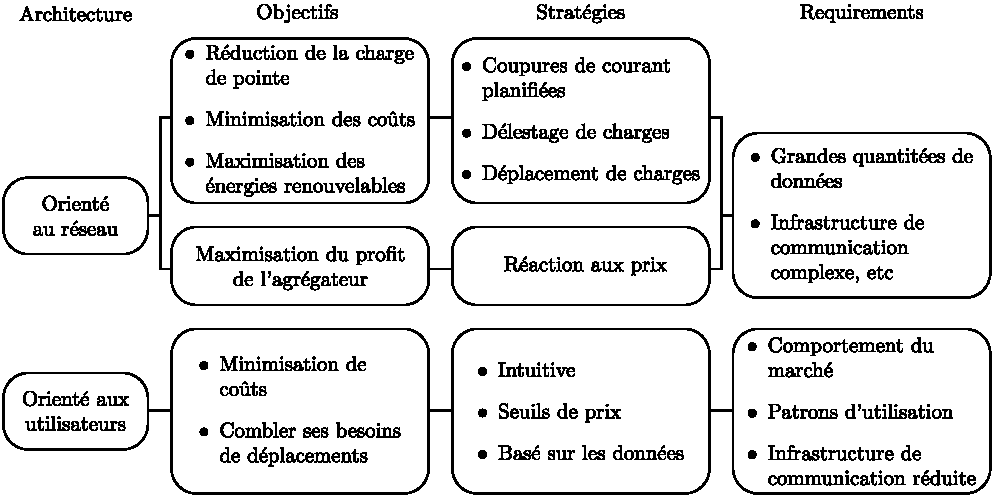
\includegraphics[width=\linewidth]{figConcMapFr.pdf}
%\end{figure}
% % \includegraphics<1>[width=0.6\linewidth]{previsiondemande.jpg}
% % \includegraphics[width=0.8\linewidth]{picos.pdf}\\
% \includegraphics[width=0.8\linewidth]{fig/picos.pdf}\\
% \tiny{Source: Report on the Economic and Environmental Impacts of Large-Scale Introduction on EV/PHEV. Shakoor and Aunedi, 2011}
% % \caption*{\only<1>{}\only<2>{\tiny Source: Report on the Economic and Environmental Impacts of Large-Scale Introduction on EV/PHEV. Shakoor $\&$ Aunedi, 2011}}
% \end{figure} 
% %{\tiny Source: Inauguration of the European Interoperability Centre for Electric Vehicles and Smart Grids}
% \end{center}

\end{frame}
% 

\begin{frame}
\frametitle{Stratégies pour la gestion de la demande}
\begin{columns}[T]
\begin{column}[T]{0.5\linewidth}
\begin{overlayarea}{0.95\linewidth}{2.8in}
\only<1->{
\begin{block}{Contrôle direct} 
\vspace{1mm}
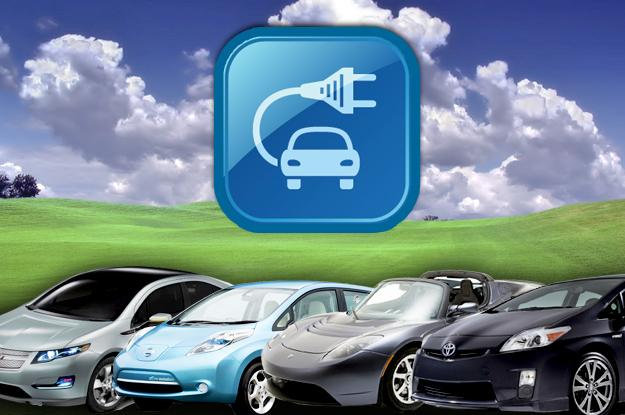
\includegraphics[width=\linewidth]{elNet.jpg}
\end{block}
}
\end{overlayarea}
\end{column}

\begin{column}[T]{0.5\linewidth}  %%<--- here
\begin{overlayarea}{0.95\linewidth}{2.8in}
\only<2->{
\begin{block}{Tarification dynamique} 
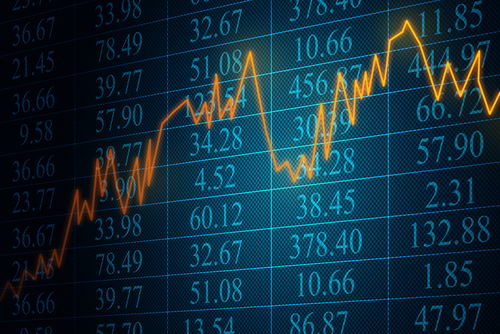
\includegraphics[width=\linewidth]{mb.jpg}
\end{block}
}
\end{overlayarea}
\end{column}
\end{columns}
\end{frame}


\begin{frame}
\begin{center}
\frametitle{Tarification dynamique}
\includegraphics<1>[width=\linewidth]{hydroquebec.jpg}
\end{center}
\end{frame}

\begin{frame}
\begin{center}
\huge \textbf{Optimiser la recharge de véhicules électriques avec une perspective utilisateur}
\end{center}
\end{frame}


\begin{frame}{Données disponibles}
\begin{center}

\includegraphics[width=0.25\linewidth]{dollarelectricity}\hspace{0.2\linewidth}

\includegraphics[width=0.25\linewidth]{cadran}


\includegraphics[width=0.25\linewidth]{event-date-and-time-symbol}\hspace{0.2\linewidth}

\includegraphics[width=0.25\linewidth]{partly-cloudy-day}
\end{center}
\end{frame}


\begin{frame}{Approches d'apprentissage disponibles}
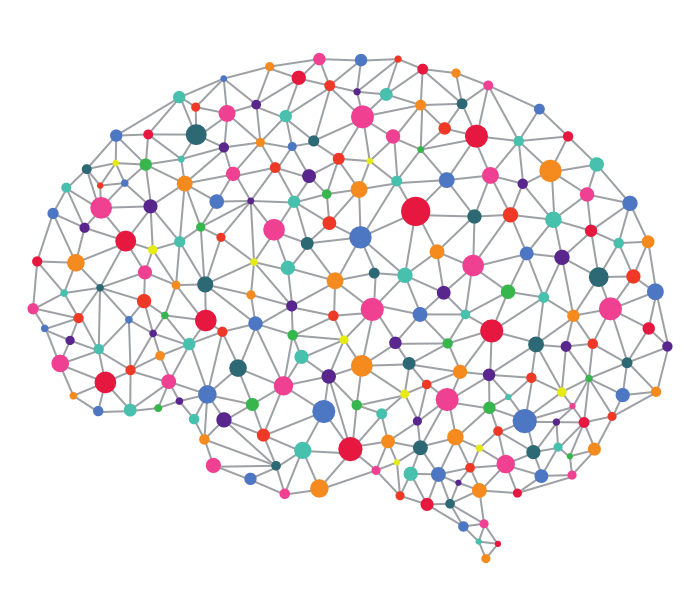
\includegraphics[width=0.7\linewidth]{neuralnet_stylised-1}
\end{frame}



\begin{frame}{Méthodologie générale}
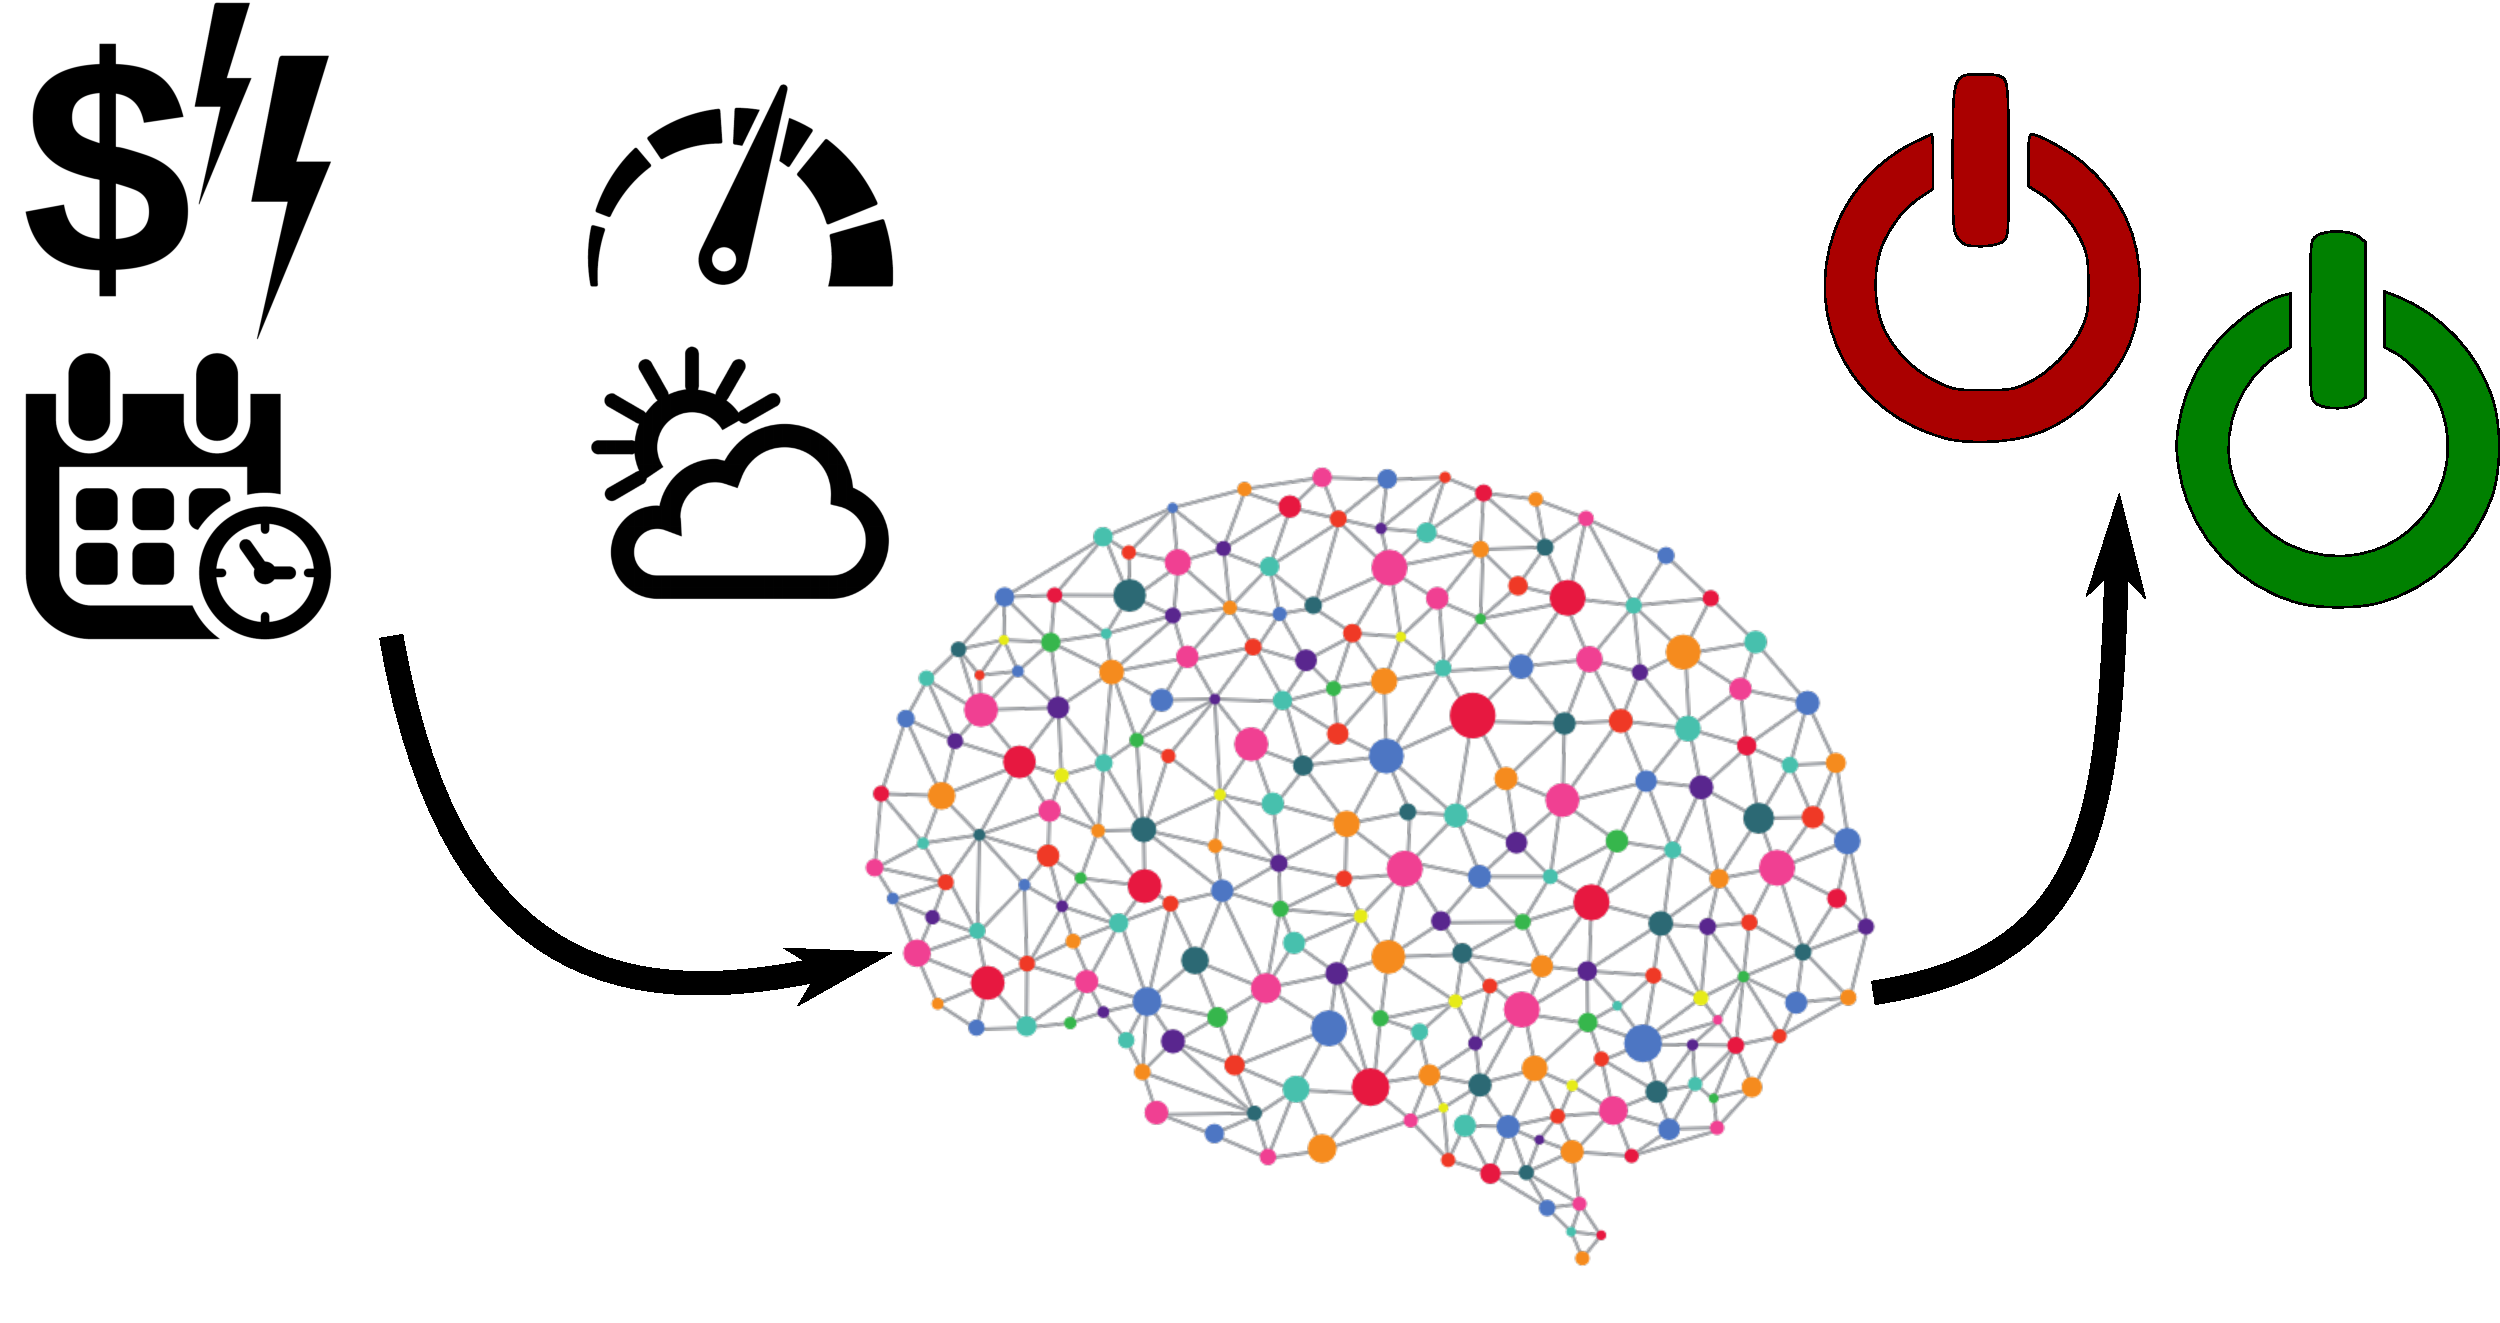
\includegraphics[width=\linewidth]{schema-global}
\end{frame}

\begin{frame}{Méthodologie générale}
\begin{enumerate}
	\item Obtenir et analyser les données pertinentes
	\item Déterminer les décisions optimales correspondantes
	\item Proposer une méthode d'apprentissage capable d'approcher les décisions optimales
\end{enumerate}
\end{frame}


\section{Analyse des données}

\begin{frame}
\begin{center}
\huge \textbf{Obtenir et analyser les données pertinentes}
\end{center}
\end{frame}

\subsection{Analyse univariée des données}
\begin{frame}
\frametitle{Analyses univariées des données} 
\begin{overlayarea}{\linewidth}{2.8in}
\begin{center} 
\includegraphics<1 | handout:0>[width=0.78\linewidth]{figUnivAnlFr1.pdf} 
\includegraphics<2 | handout:0>[width=0.78\linewidth]{figUnivAnlFr2.pdf}
\includegraphics<3 | handout:0>[width=0.78\linewidth]{figUnivAnlFr3.pdf}
\end{center}
\end{overlayarea}
\end{frame}

\subsection{Analyse multivariée des données}
\begin{frame}
\frametitle{Analyses multivariées des données - Corrélation et ACP} 

\begin{table}[t!]
\begin{center}
\centering
\scalebox{0.65}{
\begin{tabular}{lccccc}
\toprule
{} & \textbf{Température} & \textbf{Énergie consommée} & \textbf{Prix de l'essence} & \textbf{HOD} & \textbf{HOEP} \\
\midrule
\textbf{Température}   	& \x1.00&0.02	&\B{0.81}	&$-$0.02	&0.15	\\
\textbf{Énergie consommée}    & 	&1.00	&0.02	&\x0.06		&0.06	\\
\textbf{Prix de l'essence} & 	&	&1.00	&$-$0.00	&0.17	\\
\textbf{HOD}            & 	& 	&	&\x1.00		&\B{0.71}	\\
\textbf{HOEP}           & 	&	&	&		&1.00	\\
\bottomrule
\end{tabular}
}
\end{center}
\end{table}

\pause

\begin{table}
\begin{center}
\centering
\scalebox{0.65}{
\begin{tabular}{lcccccc}
\toprule
{} & \textbf{1$^{\mbox{st}}$} & \textbf{2$^{\mbox{nd}}$} & 
\textbf{3$^{\mbox{rd}}$} & \textbf{4$^{\mbox{th}}$} & \textbf{5$^{\mbox{th}}$} \\
\midrule
\textbf{Température}   &0.57&$-$0.41&$-$0.01&$-$0.06&\x0.71\\
\textbf{Énergie consommée}    &0.08&\x0.08&\x0.99&\x0.01&\x0.00\\
\textbf{Prix de l'essence} &0.58&$-$0.40&$-$0.02&$-$0.10&$-$0.71\\
\textbf{HOD}                &0.35&\x0.63&$-$0.07&$-$0.69&\x0.03\\
\textbf{HOEP}              &0.47&\x0.52&$-$0.09&\x0.71&$-$0.01\\
\bottomrule
\end{tabular}
}
\end{center}
\end{table}
\end{frame}


\begin{frame}
\frametitle{Définition du Système d'Information} 


\begin{itemize}
\item HOEP ($\ve{x}^1$), HOD ($\ve{x}^2$), et température extérieur ($\ve{x}^3$) with 101 décalages.
\item énergie consommée ($\ve{x}^4$) avec 199 décalages.
\item variables scalaires : 
\begin{itemize}
\item $w_1:$ jour de la semaine,
\item $w_2:$ heure;
\item $w_3: C_\mathit{el}(t-1)-C_\mathit{el}(t)$ différence du prix de l'électricité,
\item $w_4: C_\mathit{el}(t)$ prix de l'électricité au temps $t$ [\$/kWh],
\item $w_5: C_\mathit{fuel}(t)$ prix de l’essence au temps $t$[\$/l],
\item $w_6: dis(t)$ distance parcourue au temps $t$ [km].
\end{itemize}
\end{itemize}

\pause
... et l'état de charge du véhicule ainsi que les décisions optimales obtenues avec la programmation dynamique.

\end{frame}

\begin{frame}
\frametitle{ACP du Système d'Information} 
\begin{figure}
\begin{center}
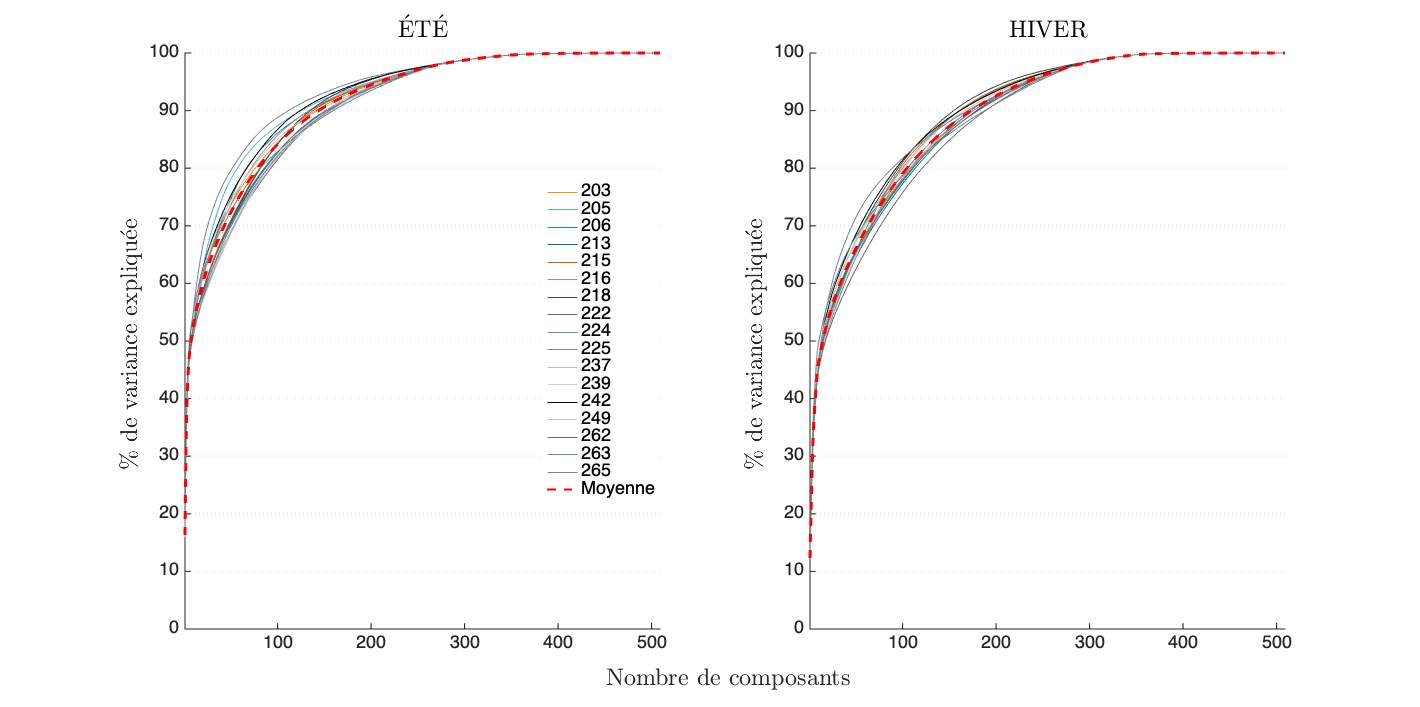
\includegraphics[width=0.99\textwidth]{figPCAvarExplainedFr.png}
\end{center}
\end{figure}
\end{frame}


\section{Stratification des données}
\subsection{Méthode pour la stratification de données}
\begin{frame}
\frametitle{Stratification des données} 
\begin{figure}
\begin{center}
\includegraphics<1>[width=0.9\linewidth]{figClusteringTrainingFr_222_summer1.pdf}
\includegraphics<2>[width=0.9\linewidth]{figStratEstimFr_222_summer1.pdf}
\end{center}
\end{figure}
\end{frame}
% 
\begin{frame}
\frametitle{Stratification dans un problème de régression avec réseau de neurones} 
\begin{figure}
\begin{center}
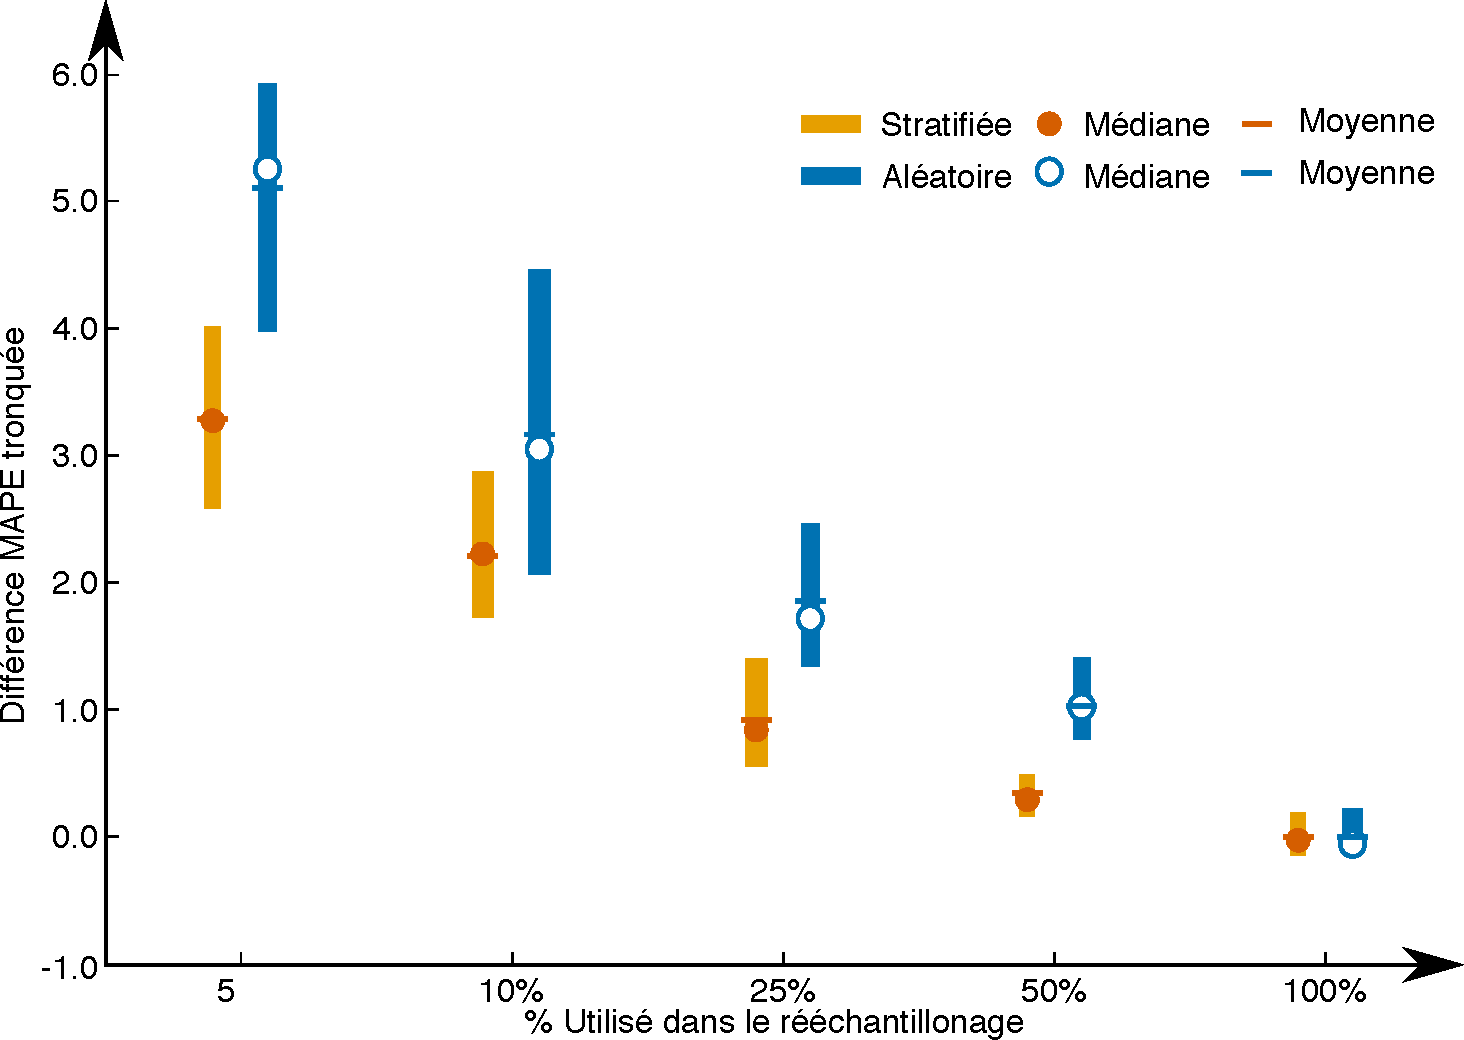
\includegraphics[width=0.7\textwidth]{figDiff_ANN_Inp_state_year_2003.pdf}
\end{center}
\end{figure}
\end{frame}

\begin{frame}
\frametitle{Stratification dans un problème de régression avec machines à vecteurs de support} 
\begin{figure}
\begin{center}
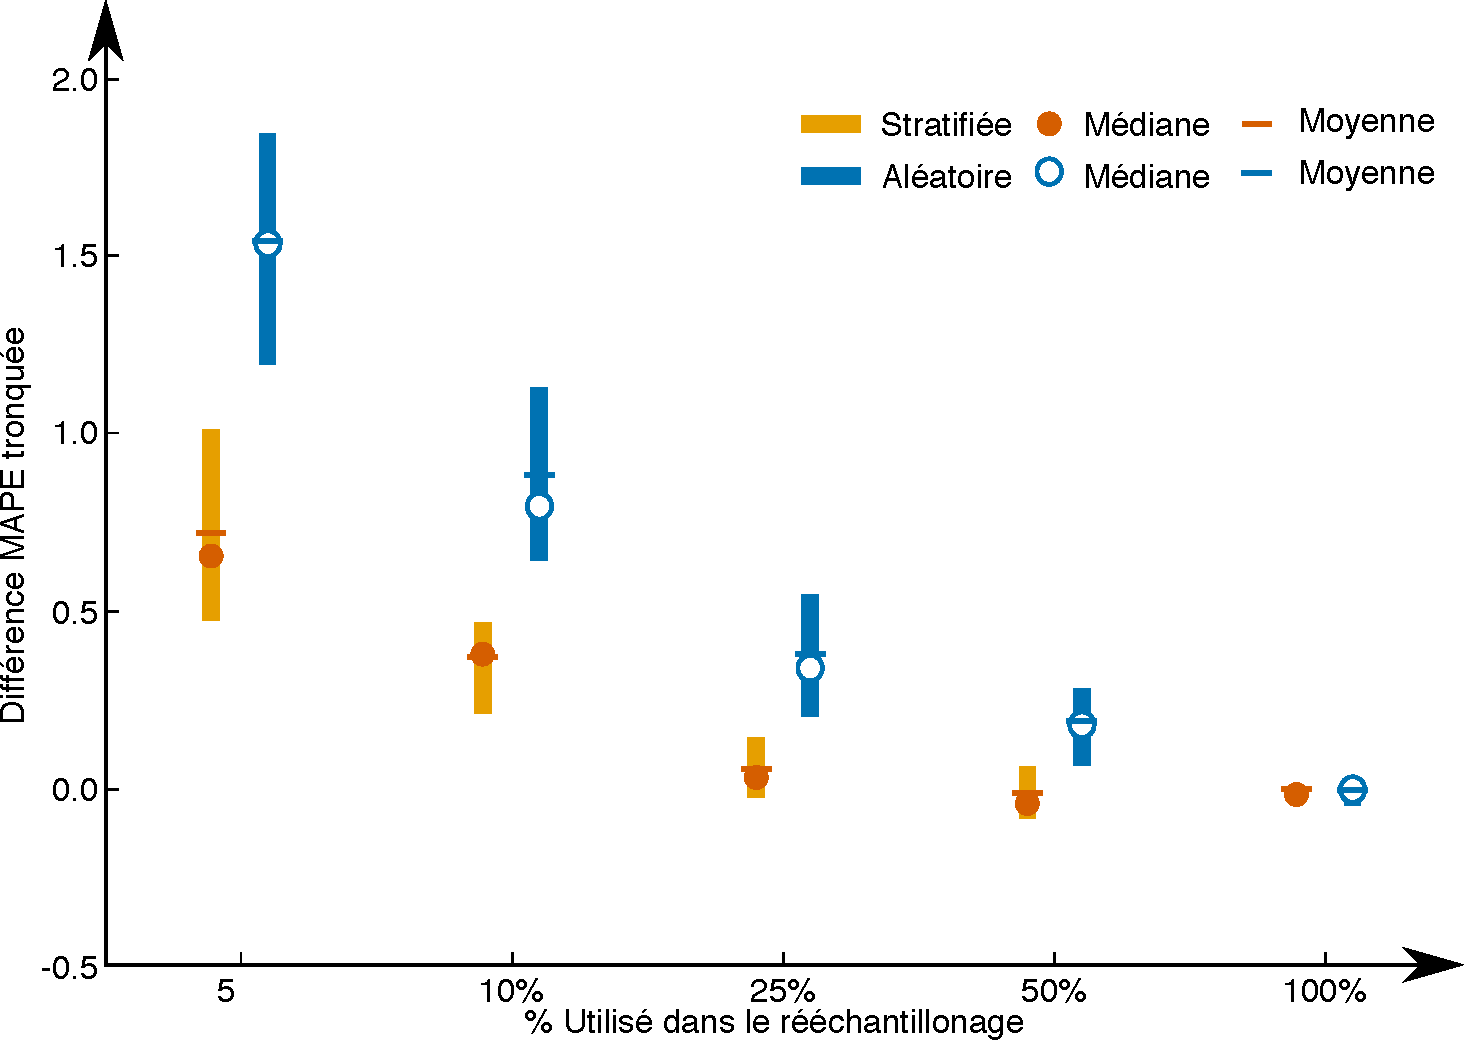
\includegraphics[width=0.7\textwidth]{figDiff_SVR_Inp_state_year_2003.pdf}
\end{center}
\end{figure}
\end{frame}




\begin{frame}
\begin{center}
\huge \textbf{Déterminer les périodes de recharge optimales}
\end{center}
\end{frame}


\subsection{Définition de la problématique}


\begin{frame}
\begin{center}
\frametitle{Programmation des périodes de recharge}
\includegraphics<1>[width=0.9\linewidth]{obj01.pdf}
\includegraphics<2>[width=0.9\linewidth]{obj02.pdf}
\includegraphics<3>[width=0.9\linewidth]{obj03.pdf}
\end{center}
\end{frame}


\begin{frame}
\frametitle{Si on suppose qu'on connaît le futur?}
\begin{center}
\begin{figure}
% 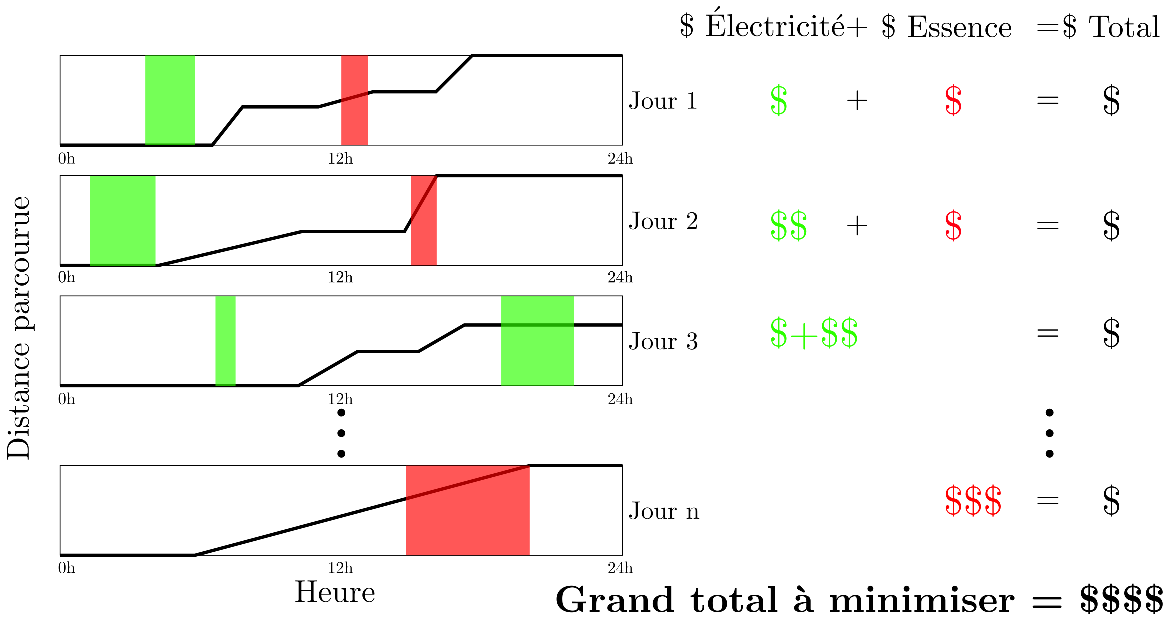
\includegraphics[width=\linewidth]{minFct.pdf}
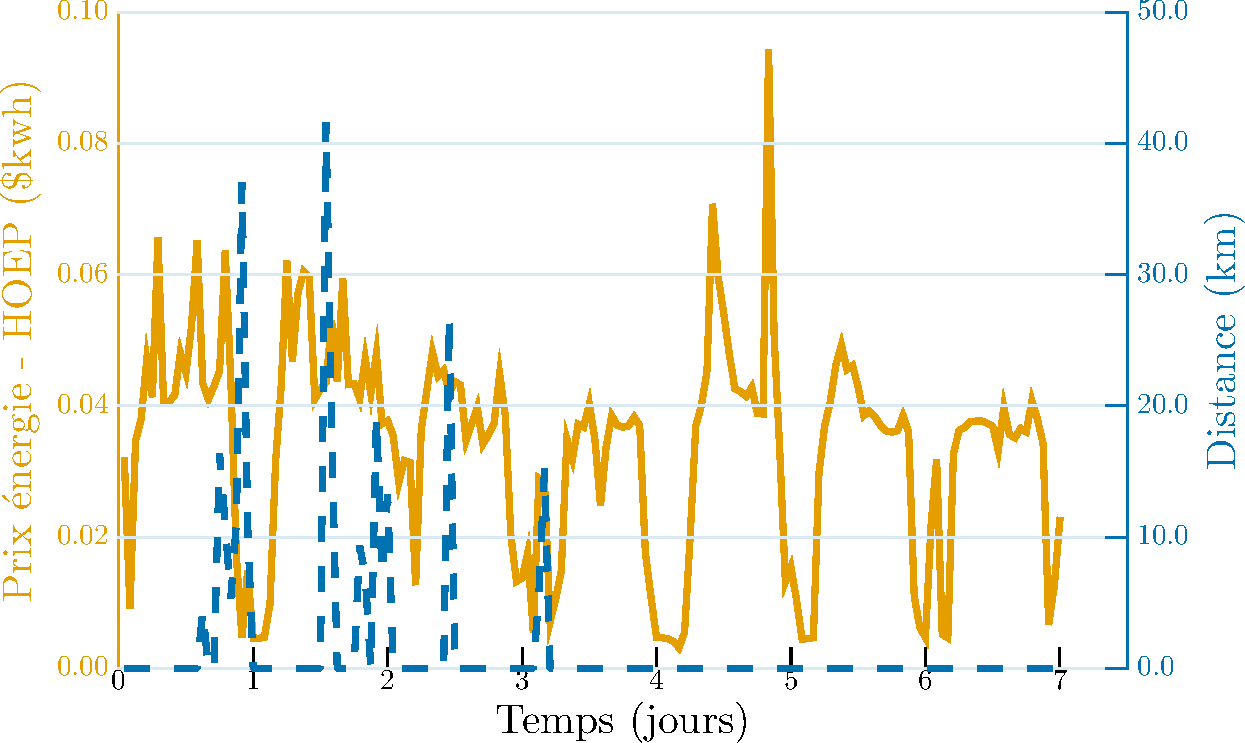
\includegraphics[width=\linewidth]{PriceDist_201Fr.pdf}
\end{figure} 
 \end{center}
\end{frame}

\begin{frame}{Formulation du problème}

\begin{itemize}
	\item Discrétisation de la journée et des états de charge
	\item À chaque temps $t$, le véhicule peut être branché ($z(t)=1$) ou non branché ($z(t)=0$)
	\item Si branché, on peut charger ou non ($a(t) = \{0, 1\}$)
\begin{equation}\label{eq:costp1}
S_p(t) = a(t) \cdot C_{el}(t) \cdot \frac{E_{ch}(SoC(t))}{\eta}
\end{equation}
	\item Sinon, on ne peut que consommer de l'énergie
\begin{equation}\label{eq:costp2}
S_u(t) = C_{fuel}(t) \cdot \max(F_{c}(SoC(t)),0)
\end{equation}
	\item Objectif : minimiser le coût d'utilisation
\begin{equation}
\min_{\{a(t)\}_{t=1}^T}~\sum_{t=1}^{T} \left[z(t) \cdot S_p(t) + (1-z(t)) \cdot S_u(t)\right]
\label{eq:cost}
\end{equation}
\end{itemize}

\end{frame}


\begin{frame}
\frametitle{Processus de décision Markovien}
\begin{center}
\begin{itemize}
\item Les états :
 
\begin{equation}
s(t) = \frac{\lfloor \mathit{SoC}(t) \cdot B \rfloor + 0.5}{B} 
\label{eq:state}
\end{equation}
\item Les actions ($a=0$, $a=1$)
\item La fonction de transition (modèle de batterie)
\item La fonction de récompense :
\begin{equation}
r(s(t),a) =
\begin{cases}
0 & \text{si $z(t)=1$ et $a=0$}\\
-C_{el}(t) \cdot \frac{E_{ch}(SoC(t))}{\eta} & \text{si $z(t)=1$ et $a=1$}\\
- C_{fuel}(t) \cdot F_{c}(SoC(t)) & \text{si $z(t)=0$}   
\end{cases}.\label{eq:reward}
\end{equation}
\end{itemize}
\end{center}
\end{frame}



\begin{frame}
\begin{center}
\frametitle{Optimisation basée sur la Programmation Dynamique}

\begin{equation}
Q(s(t),a) =
r(s(t),a) + \max\limits_{a\in\mathcal{A}} Q(s(t+1),a) 
\end{equation}

\begin{equation}
a^*(t) = \argmax\limits_{a\in\mathcal{A}}~Q(s(t),a).\label{eq:adecisions}
\end{equation}
\end{center}
\end{frame}


\begin{frame}
\frametitle{Prise de décisions avec la programmation dynamique (Exemple illustratif)}
\begin{center}
\begin{figure}
% 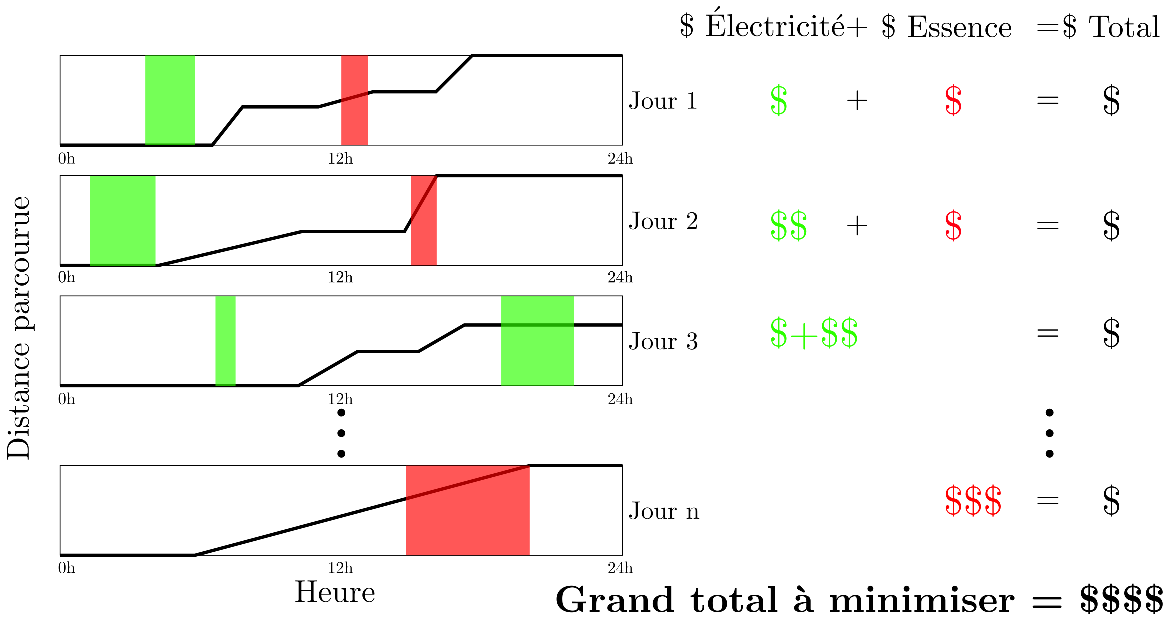
\includegraphics[width=\linewidth]{minFct.pdf}
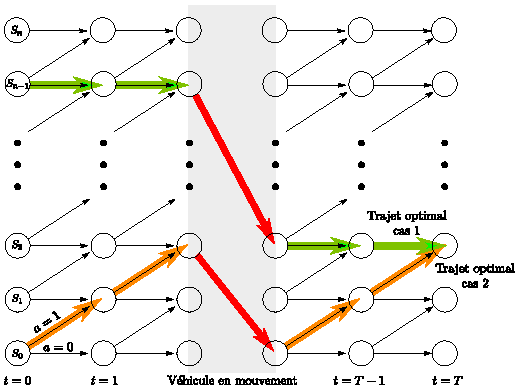
\includegraphics[width=0.7\linewidth]{figDinamycProgram02.pdf}
\end{figure} 
 \end{center}
\end{frame}


\begin{frame}
\frametitle{Analyse de l'intervalle de temps}
\begin{center}
\begin{figure}
% 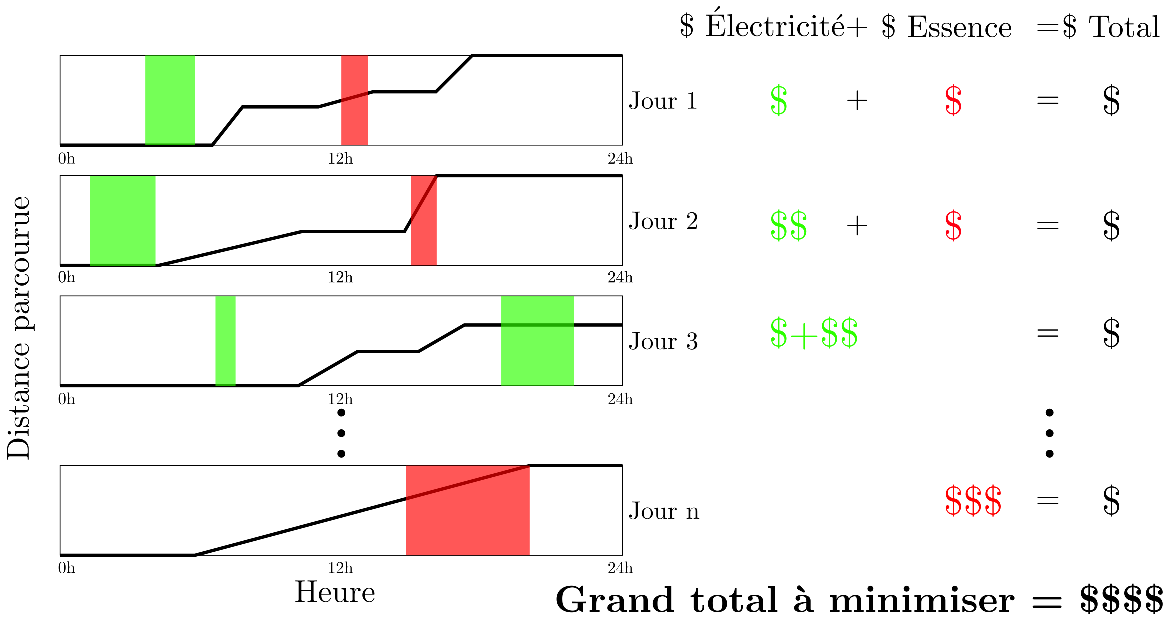
\includegraphics[width=\linewidth]{minFct.pdf}
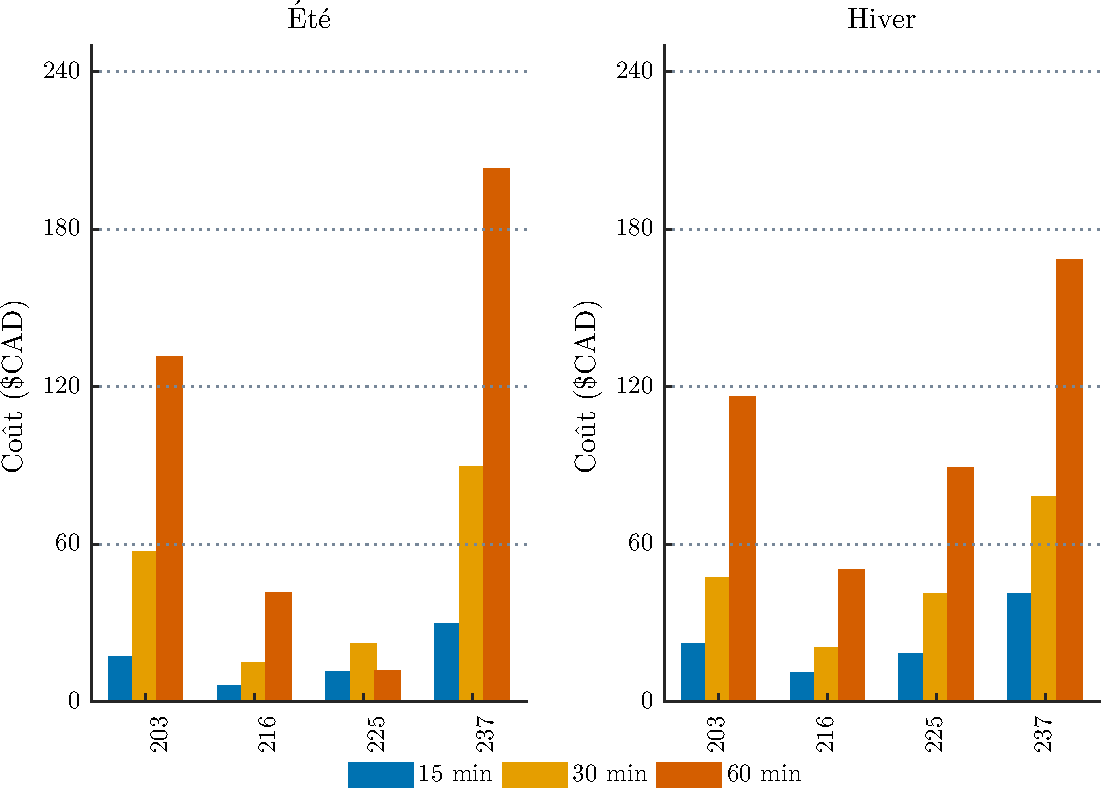
\includegraphics[width=0.9\linewidth]{figresDeltaWithoutGasBWcolor02-Sout2.pdf}
\end{figure} 
 \end{center}
\end{frame}

\subsection{Résultats obtenus avec la programmation dynamique}

\begin{frame}
\begin{center}
\frametitle{Résultats}

% \begin{table}[t!]
% \begin{center}
% \caption[Cost and gain of \gls{dp}, \gls{ac}, and \gls{rd} models in summer and winter.]{Cost and gain regarding the \gls{gas} in relation of \gls{dp}, \gls{ac}, and \gls{rd} models in summer and winter test datasets, for the 17 \glspl{ev} evaluated. Values corresponding to the cost ($\$$) are related to the energy cost of the usage during the period, while values given as percentage ($\%$) correspond to the gain of the each strategy compared to driving only with \gls{gas}.}
% \label{t:ACmodel}
\scalebox{0.8}{
\begin{tabular}{ccccccccc}
\toprule
\multirow{3}{*}{} & \multicolumn{7}{c}{\B{Hiver}} &  \\
 & \B{Essence} & \multicolumn{2}{c}{\B{Prog. dynamique}} & \multicolumn{2}{c}{\B{Charge toujours}} & \multicolumn{2}{c}{\B{RD}} & \\
 \cmidrule(lr){3-4} \cmidrule(lr){5-6} \cmidrule(lr){7-8} 
 {} & \B{\$} & \B{\$} & \B{\%} & \B{\$} & \B{\%} & \B{\$} & \B{\%} & {}  \\
\midrule 
% 203 & 131.2 & 34.0 & 74 & \s91.0 & 31 & \s93.7 & 29 & & \s65.1 & \s7.9 & 88 & \s29.1 & 55 & \s30.1 & 54 \\
% 205 & \s93.0 & 22.1 & 76 & \s57.4 & 38 & \s57.1 & 39 & & \s45.5 & \s5.4 & 88 & \s22.2 & 51 & \s24.8 & 45 \\
% 206 & \s52.4 & \s1.5 & 97 & \s16.4 & 69 & \s14.6 & 72 & & \s34.9 & \s5.5 & 84 & \s20.5 & 41 & \s21.4 & 39 \\
% 213 & 187.4 & 15.7 & 92 & \s60.6 & 68 & \s60.4 & 68 & & \s66.5 & \s7.4 & 89 & \s27.2 & 59 & \s28.7 & 57 \\
% 215 & 230.8 & 66.8 & 71 & 165.6 & 28 & 184.1 & 20 & & \s58.8 & \s6.3 & 89 & \s24.6 & 58 & \s25.2 & 57 \\
% 216 & \s93.2 & \s3.3 & 96 & \s24.7 & 73 & \s23.9 & 74 & & \s79.2 & 19.4 & 76 & \s55.8 & 29 & \s59.1 & 25 \\
% 218 & \s81.0 & \s3.2 & 96 & \s21.4 & 74 & \s20.7 & 74 & & \s40.5 & \s4.2 & 90 & \s18.3 & 55 & \s18.8 & 53 \\
% 222 & \s66.5 & \s3.0 & 95 & \s21.0 & 68 & \s21.9 & 67 & & \s42.9 & \s4.6 & 89 & \s19.3 & 55 & \s20.8 & 52 \\
% 224 & 228.4 & 87.1 & 62 & 207.2 & \s9 & 220.8 & \s3 & & \s31.9 & \s2.8 & 91 & \s13.8 & 57 & \s13.1 & 59 \\
% 225 & \s64.4 & \s1.4 & 98 & \s17.7 & 73 & \s15.8 & 75 & & \s66.0 & \s8.4 & 87 & \s28.1 & 57 & \s29.9 & 55 \\
% 237 & 156.8 & 17.3 & 89 & \s56.5 & 64 & \s63.0 & 60 & & 108.3 & 14.2 & 87 & \s44.4 & 59 & \s47.4 & 56 \\
% 239 & \s72.2 & \s2.5 & 97 & \s23.3 & 68 & \s22.0 & 70 & & \s64.2 & \s7.4 & 88 & \s26.4 & 59 & \s28.5 & 56 \\
% 242 & 364.3 & 98.0 & 73 & 232.5 & 36 & 287.3 & 21 & & 178.0 & 49.6 & 72 & 133.8 & 25 & 150.1 & 16 \\
% 249 & 122.1 & \s5.0 & 96 & \s34.9 & 71 & \s32.9 & 73 & & \s36.1 & \s3.6 & 90 & \s15.1 & 58 & \s15.9 & 56 \\
% 262 & \s20.8 & \s0.4 & 98 & \s\s6.2 & 70 & \s\s5.8 & 72 & & \s61.8 & \s6.4 & 90 & \s25.8 & 58 & \s27.2 & 56 \\
% 263 & \s32.0 & \s2.3 & 93 & \s\s9.6 & 70 & \s\s8.3 & 74 & & \s52.8 & \s7.2 & 86 & \s23.0 & 56 & \s24.7 & 53 \\
% 265 & \s57.7 & \s1.6 & 97 & \s17.3 & 70 & \s15.7 & 73 & & \s23.8 & \s2.4 & 90 & \s10.9 & 54 & \s11.1 & 53 \\
\B{Moyenne} &  \B{\s62.1} & \B{\s9.6} & \B{87} & \B{\s31.7} & \B{52} & \B{\s33.9} & \B{50} \\
\B{Médiane} &  \B{\s58.8} & \B{\s6.4} & \B{88} & \B{\s24.6} & \B{56} & \B{\s25.2} & \B{54} \\
\bottomrule    
\end{tabular}
}

\vspace*{25px}


\scalebox{0.8}{
\begin{tabular}{ccccccccc}
\toprule
\multirow{3}{*}{} & \multicolumn{7}{c}{\B{Été}} &  \\
 & \B{Essence} & \multicolumn{2}{c}{\B{Prog. dynamique}} & \multicolumn{2}{c}{\B{Charge toujours}} & \multicolumn{2}{c}{\B{RD}} & \\
 \cmidrule(lr){3-4} \cmidrule(lr){5-6} \cmidrule(lr){7-8} 
 {} & \B{\$} & \B{\$} & \B{\%} & \B{\$} & \B{\%} & \B{\$} & \B{\%} & {}  \\
\midrule 
% 203 & 131.2 & 34.0 & 74 & \s91.0 & 31 & \s93.7 & 29 & & \s65.1 & \s7.9 & 88 & \s29.1 & 55 & \s30.1 & 54 \\
% 205 & \s93.0 & 22.1 & 76 & \s57.4 & 38 & \s57.1 & 39 & & \s45.5 & \s5.4 & 88 & \s22.2 & 51 & \s24.8 & 45 \\
% 206 & \s52.4 & \s1.5 & 97 & \s16.4 & 69 & \s14.6 & 72 & & \s34.9 & \s5.5 & 84 & \s20.5 & 41 & \s21.4 & 39 \\
% 213 & 187.4 & 15.7 & 92 & \s60.6 & 68 & \s60.4 & 68 & & \s66.5 & \s7.4 & 89 & \s27.2 & 59 & \s28.7 & 57 \\
% 215 & 230.8 & 66.8 & 71 & 165.6 & 28 & 184.1 & 20 & & \s58.8 & \s6.3 & 89 & \s24.6 & 58 & \s25.2 & 57 \\
% 216 & \s93.2 & \s3.3 & 96 & \s24.7 & 73 & \s23.9 & 74 & & \s79.2 & 19.4 & 76 & \s55.8 & 29 & \s59.1 & 25 \\
% 218 & \s81.0 & \s3.2 & 96 & \s21.4 & 74 & \s20.7 & 74 & & \s40.5 & \s4.2 & 90 & \s18.3 & 55 & \s18.8 & 53 \\
% 222 & \s66.5 & \s3.0 & 95 & \s21.0 & 68 & \s21.9 & 67 & & \s42.9 & \s4.6 & 89 & \s19.3 & 55 & \s20.8 & 52 \\
% 224 & 228.4 & 87.1 & 62 & 207.2 & \s9 & 220.8 & \s3 & & \s31.9 & \s2.8 & 91 & \s13.8 & 57 & \s13.1 & 59 \\
% 225 & \s64.4 & \s1.4 & 98 & \s17.7 & 73 & \s15.8 & 75 & & \s66.0 & \s8.4 & 87 & \s28.1 & 57 & \s29.9 & 55 \\
% 237 & 156.8 & 17.3 & 89 & \s56.5 & 64 & \s63.0 & 60 & & 108.3 & 14.2 & 87 & \s44.4 & 59 & \s47.4 & 56 \\
% 239 & \s72.2 & \s2.5 & 97 & \s23.3 & 68 & \s22.0 & 70 & & \s64.2 & \s7.4 & 88 & \s26.4 & 59 & \s28.5 & 56 \\
% 242 & 364.3 & 98.0 & 73 & 232.5 & 36 & 287.3 & 21 & & 178.0 & 49.6 & 72 & 133.8 & 25 & 150.1 & 16 \\
% 249 & 122.1 & \s5.0 & 96 & \s34.9 & 71 & \s32.9 & 73 & & \s36.1 & \s3.6 & 90 & \s15.1 & 58 & \s15.9 & 56 \\
% 262 & \s20.8 & \s0.4 & 98 & \s\s6.2 & 70 & \s\s5.8 & 72 & & \s61.8 & \s6.4 & 90 & \s25.8 & 58 & \s27.2 & 56 \\
% 263 & \s32.0 & \s2.3 & 93 & \s\s9.6 & 70 & \s\s8.3 & 74 & & \s52.8 & \s7.2 & 86 & \s23.0 & 56 & \s24.7 & 53 \\
% 265 & \s57.7 & \s1.6 & 97 & \s17.3 & 70 & \s15.7 & 73 & & \s23.8 & \s2.4 & 90 & \s10.9 & 54 & \s11.1 & 53 \\
\B{Moyenne} & \B{120.8} & \B{\s21.5} & \B{88} & \B{\s62.6} & \B{58} & \B{\s67.5} & \B{57} &   \\
\B{Médiane} & \B{\s93.0} & \B{\s3.3} & \B{96} & \B{\s24.7} & \B{68} & \B{\s23.9} & \B{70} &  \\
\bottomrule    
\end{tabular}
}

% \end{center}
% \end{table}
\end{center}
\end{frame}



\section{Système d'information}
\subsection{Analyse univariée des données}
\begin{frame}
\frametitle{Analyses univariées des données} 
\begin{overlayarea}{\linewidth}{2.8in}
\begin{center} 
\includegraphics<1 | handout:0>[width=0.78\linewidth]{figUnivAnlFr1.pdf} 
\includegraphics<2 | handout:0>[width=0.78\linewidth]{figUnivAnlFr2.pdf}
\includegraphics<3 | handout:0>[width=0.78\linewidth]{figUnivAnlFr3.pdf}
\end{center}
\end{overlayarea}
\end{frame}

\subsection{Analyse multivariée des données}
\begin{frame}
\frametitle{Analyses multivariées des données - Corrélation et ACP} 

\begin{table}[t!]
\begin{center}
\centering
\scalebox{0.65}{
\begin{tabular}{lccccc}
\toprule
{} & \textbf{Température} & \textbf{Énergie consommée} & \textbf{Prix de l'essence} & \textbf{HOD} & \textbf{HOEP} \\
\midrule
\textbf{Température}   	& \x1.00&0.02	&\B{0.81}	&$-$0.02	&0.15	\\
\textbf{Énergie consommée}    & 	&1.00	&0.02	&\x0.06		&0.06	\\
\textbf{Prix de l'essence} & 	&	&1.00	&$-$0.00	&0.17	\\
\textbf{HOD}            & 	& 	&	&\x1.00		&\B{0.71}	\\
\textbf{HOEP}           & 	&	&	&		&1.00	\\
\bottomrule
\end{tabular}
}
\end{center}
\end{table}

\pause

\begin{table}
\begin{center}
\centering
\scalebox{0.65}{
\begin{tabular}{lcccccc}
\toprule
{} & \textbf{1$^{\mbox{st}}$} & \textbf{2$^{\mbox{nd}}$} & 
\textbf{3$^{\mbox{rd}}$} & \textbf{4$^{\mbox{th}}$} & \textbf{5$^{\mbox{th}}$} \\
\midrule
\textbf{Température}   &0.57&$-$0.41&$-$0.01&$-$0.06&\x0.71\\
\textbf{Énergie consommée}    &0.08&\x0.08&\x0.99&\x0.01&\x0.00\\
\textbf{Prix de l'essence} &0.58&$-$0.40&$-$0.02&$-$0.10&$-$0.71\\
\textbf{HOD}                &0.35&\x0.63&$-$0.07&$-$0.69&\x0.03\\
\textbf{HOEP}              &0.47&\x0.52&$-$0.09&\x0.71&$-$0.01\\
\bottomrule
\end{tabular}
}
\end{center}
\end{table}
\end{frame}


\begin{frame}
\frametitle{Définition du Système d'Information} 


\begin{itemize}
\item HOEP ($\ve{x}^1$), HOD ($\ve{x}^2$), et température extérieur ($\ve{x}^3$) with 101 décalages.
\item énergie consommée ($\ve{x}^4$) avec 199 décalages.
\item variables scalaires : 
\begin{itemize}
\item $w_1:$ jour de la semaine,
\item $w_2:$ heure;
\item $w_3: C_\mathit{el}(t-1)-C_\mathit{el}(t)$ différence du prix de l'électricité,
\item $w_4: C_\mathit{el}(t)$ prix de l'électricité au temps $t$ [\$/kWh],
\item $w_5: C_\mathit{fuel}(t)$ prix de l’essence au temps $t$[\$/l],
\item $w_6: dis(t)$ distance parcourue au temps $t$ [km].
\end{itemize}
\end{itemize}

\pause
... et l'état de charge du véhicule ainsi que les décisions optimales obtenues avec la programmation dynamique.

\end{frame}

\begin{frame}
\frametitle{ACP du Système d'Information} 
\begin{figure}
\begin{center}
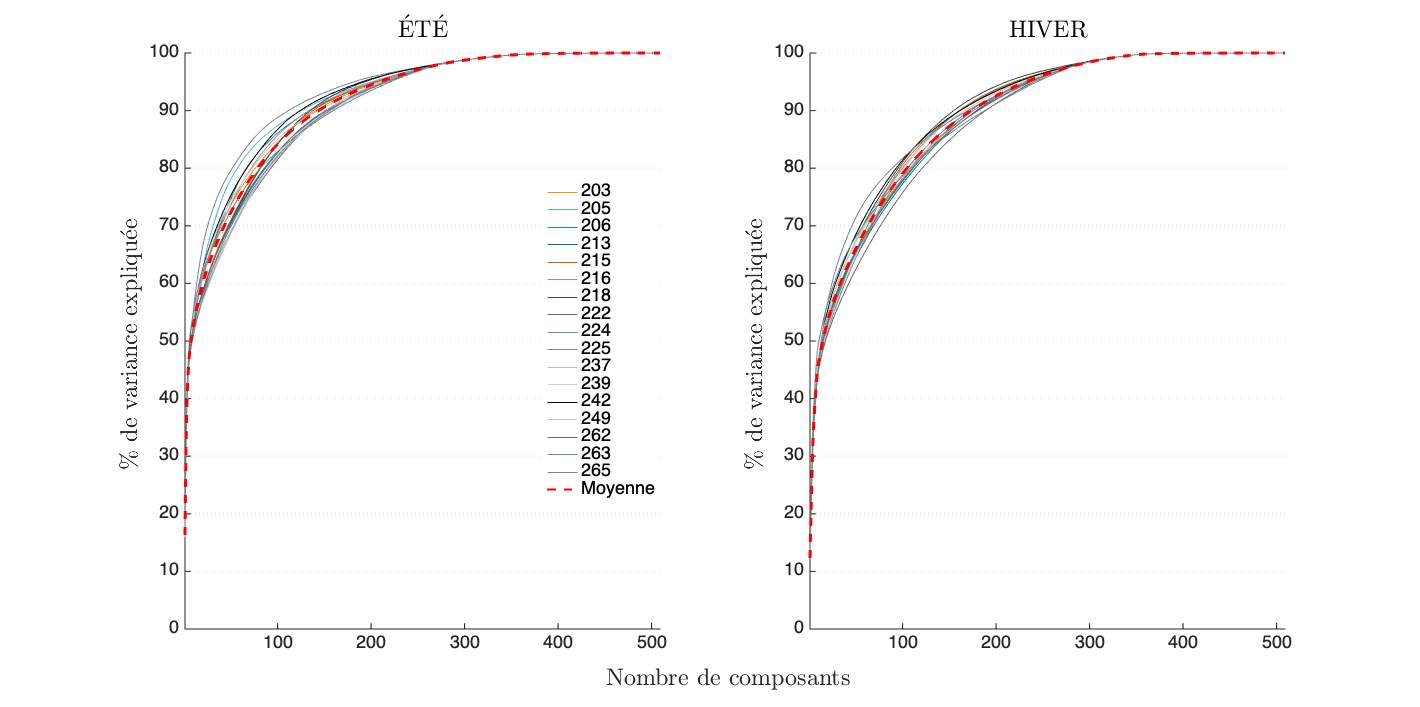
\includegraphics[width=0.99\textwidth]{figPCAvarExplainedFr.png}
\end{center}
\end{figure}
\end{frame}


\section{Stratification des données}
\subsection{Méthode pour la stratification de données}
\begin{frame}
\frametitle{Stratification des données} 
\begin{figure}
\begin{center}
\includegraphics<1>[width=0.9\linewidth]{figClusteringTrainingFr_222_summer1.pdf}
\includegraphics<2>[width=0.9\linewidth]{figStratEstimFr_222_summer1.pdf}
\end{center}
\end{figure}
\end{frame}
% 
\begin{frame}
\frametitle{Stratification dans un problème de régression avec réseau de neurones} 
\begin{figure}
\begin{center}
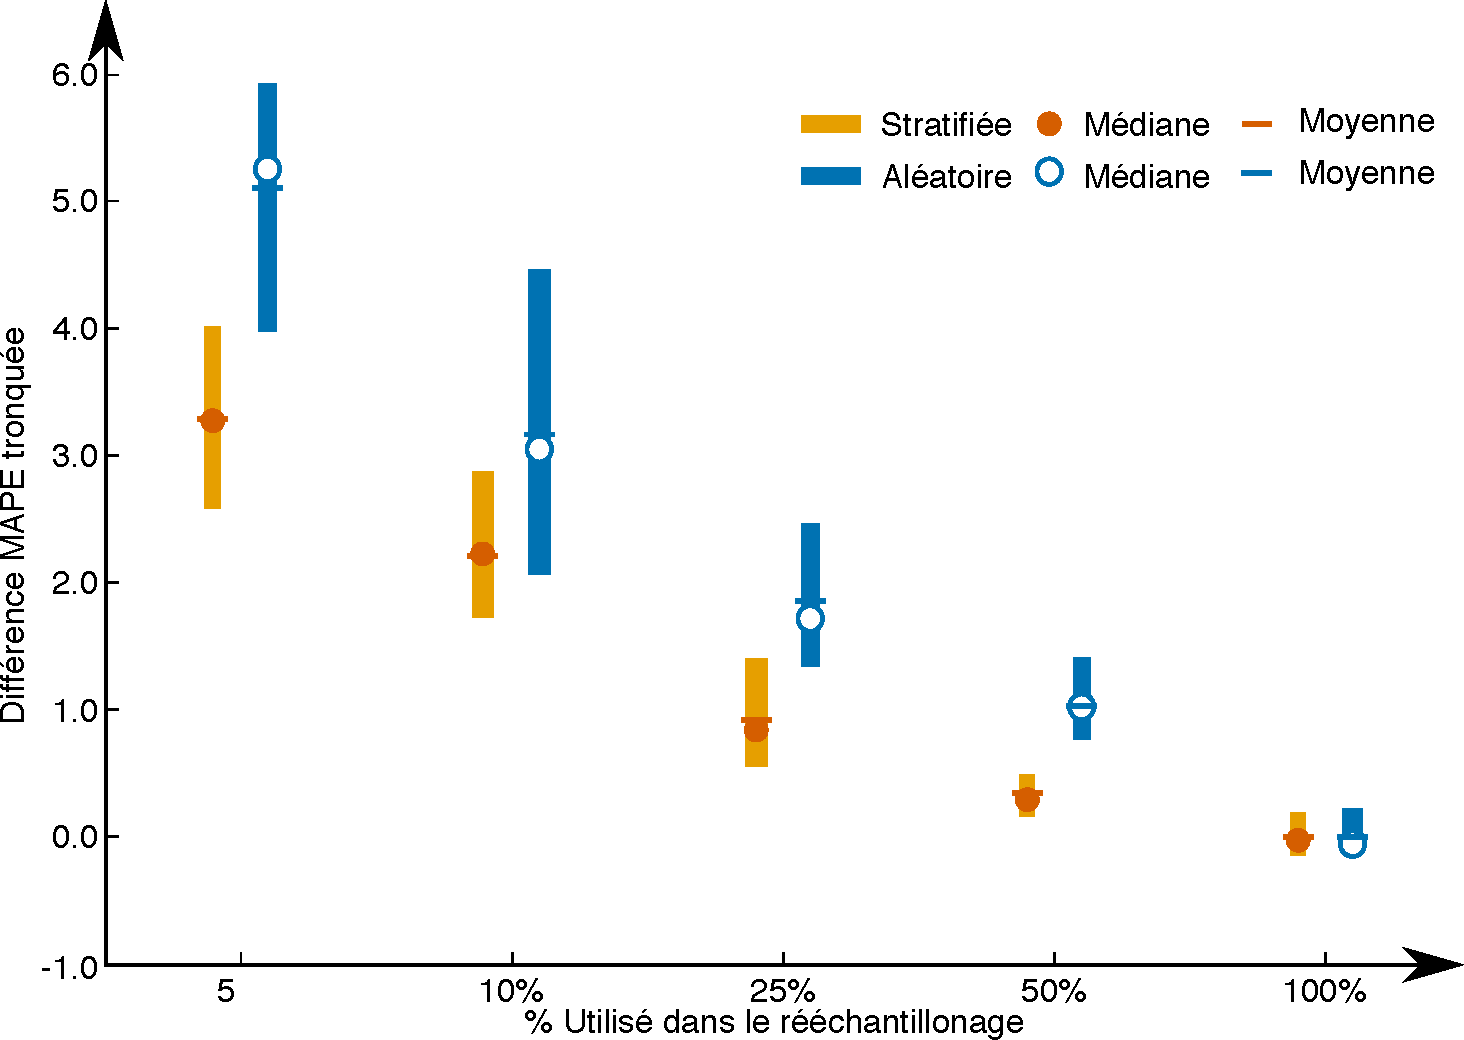
\includegraphics[width=0.7\textwidth]{figDiff_ANN_Inp_state_year_2003.pdf}
\end{center}
\end{figure}
\end{frame}

\begin{frame}
\frametitle{Stratification dans un problème de régression avec machines à vecteurs de support} 
\begin{figure}
\begin{center}
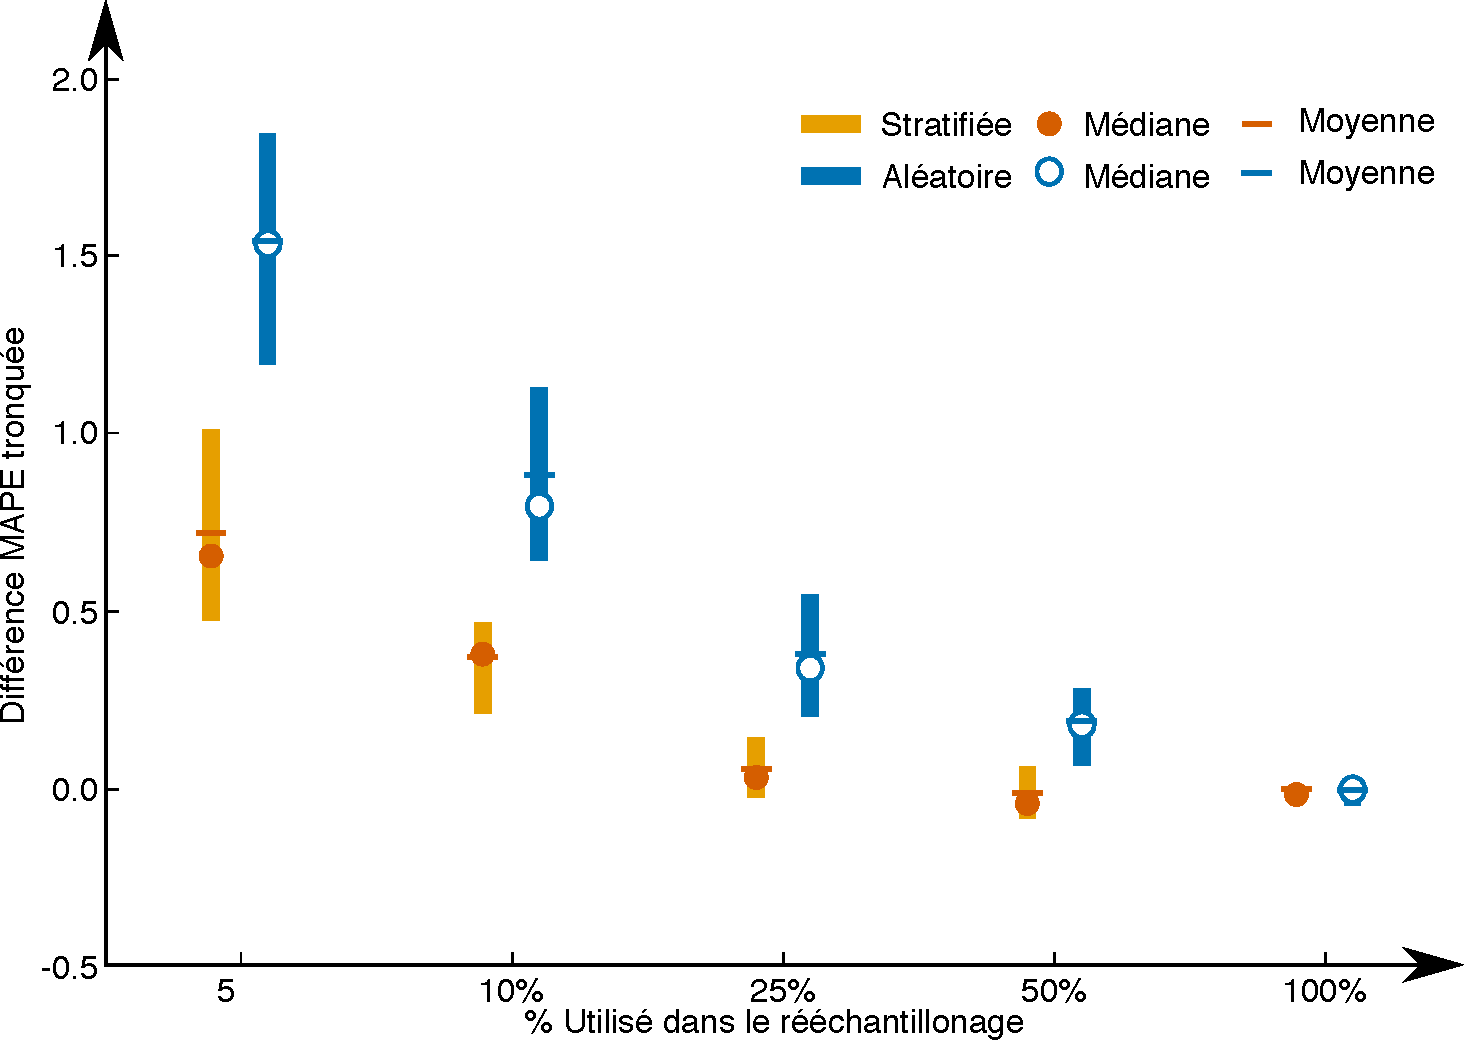
\includegraphics[width=0.7\textwidth]{figDiff_SVR_Inp_state_year_2003.pdf}
\end{center}
\end{figure}
\end{frame}
% 


\section{Recharge intelligente de VE}

\subsection{Méthodologie}


 \begin{frame}{Considérations importantes}
 \begin{itemize}
 	\item Aucune hypothèse nécessaire sur les modèles utilisés
 	\begin{itemize}
 		\item Voiture hybride rechargeable / 100\% électrique
 		\item Caractéristiques de la batterie
 		\item Caractéristiques du chargeur
 		\item Incitatifs supplémentaires (e.g. vente d'électricité)
 	\end{itemize}
 	\item La solution obtenue est \emph{globalement optimale}
 \end{itemize}
 \end{frame}
 
 


\begin{frame}
\begin{center}
%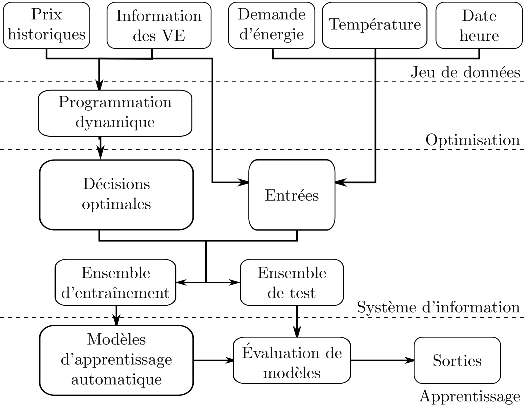
\includegraphics[width=0.7\textwidth]{artMeth2CompactFr.pdf}
\huge \textbf{Apprendre les décisions optimales}
\end{center}
\end{frame}

\begin{frame}{Pipeline d'apprentissage automatique}
\begin{itemize}
	\item Mêmes données d'entrée, sans connaître le futur
	\item Vérité terrain donnée par la programmation dynamique
	\item Techniques comparées :
	\begin{itemize}
		\item Système de régles à base de seuils
		\item k-plus proches voisins
		\item Réseaux de neurones avec de données stratifiés
		 \item Réseaux de neurones profonds
 
	\end{itemize}
\end{itemize}

\end{frame}


\begin{frame}
\frametitle{Système de régles à base de seuils} 
\begin{figure}
\begin{center}
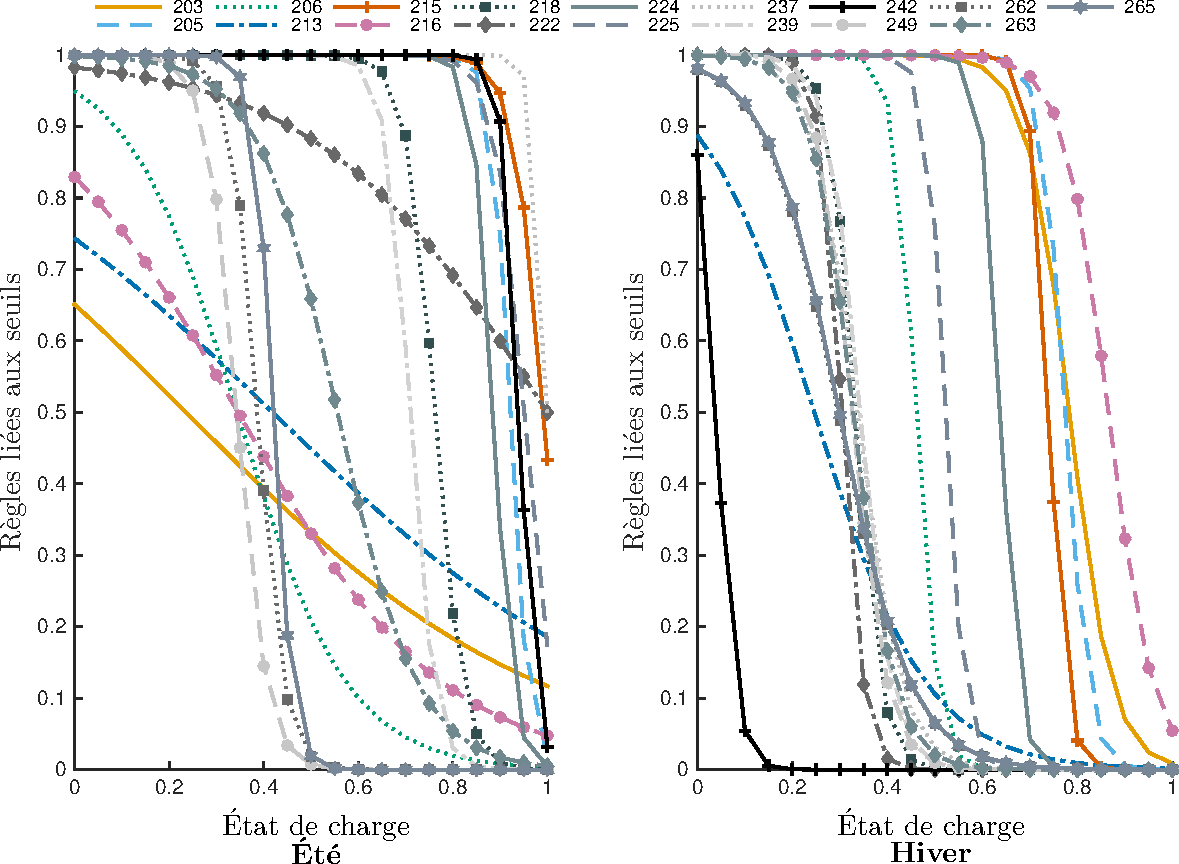
\includegraphics[width=0.9\textwidth]{figtbrFr.pdf}
\end{center}
\end{figure}
\end{frame}
% 


\begin{frame}
\frametitle{k-plus proches voisins} 
\begin{figure}
\begin{center}
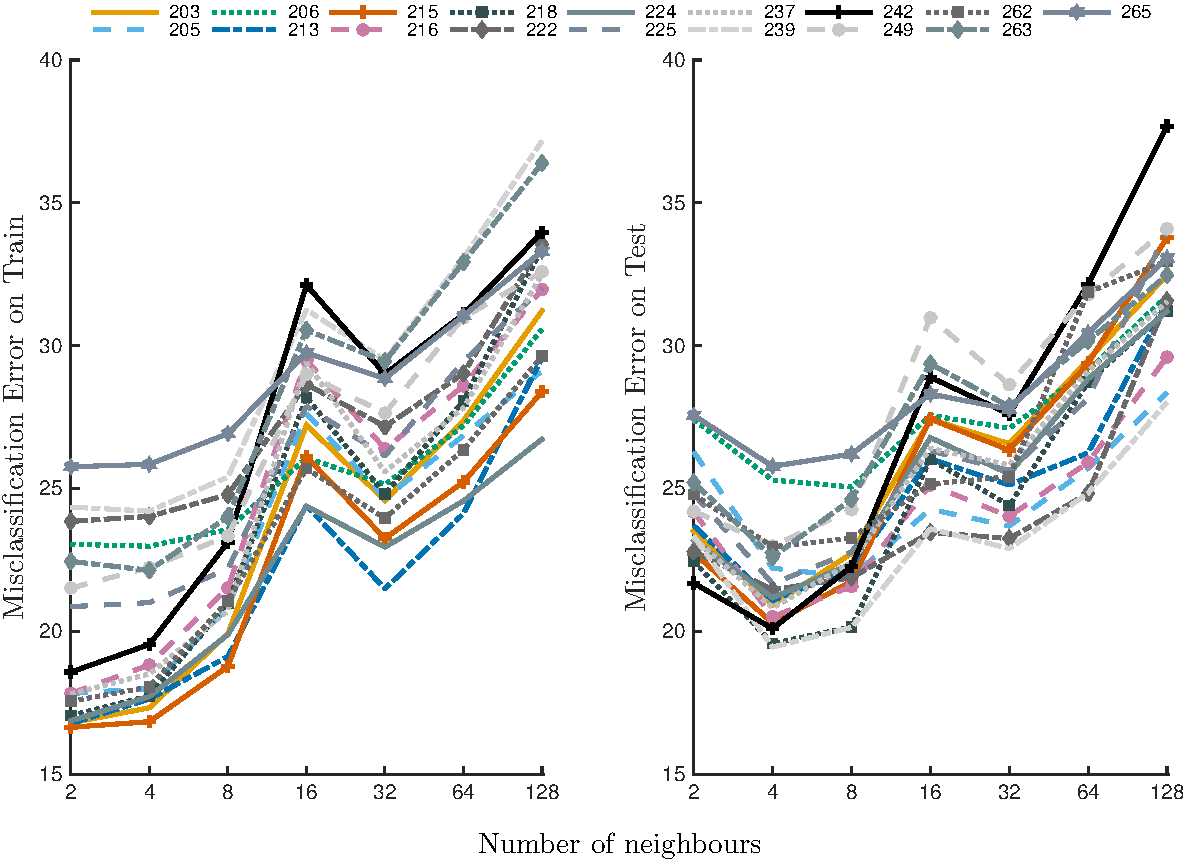
\includegraphics[width=0.9\textwidth]{figknn.pdf}
\end{center}
\end{figure}
\end{frame}
% 
% 

\subsection{Analyse des résultats}
% 
% \begin{frame}
% \begin{center}
% \begin{overlayarea}{\linewidth}{2.8in}
% \includegraphics<1 | handout:0>[width=\linewidth]{resultats01.pdf}
% \includegraphics<2 | handout:0>[width=\linewidth]{resultats02.pdf}
% \includegraphics<3>[width=\linewidth]{resultats03.pdf}
% \end{overlayarea}
% \end{center}
% \end{frame}


\begin{frame}
\begin{center}
\begin{overlayarea}{\linewidth}{2.8in}
\includegraphics<1 | handout:0>[width=\linewidth]{figResAnalysis01.pdf}
\includegraphics<2 | handout:0>[width=\linewidth]{figResAnalysis02.pdf}
\includegraphics<3>[width=\linewidth]{figResAnalysis03.pdf}
\end{overlayarea}
\end{center}
\end{frame}



\begin{frame}
\frametitle{Résultats} 
\begin{figure}
\begin{center}
\begin{overlayarea}{\linewidth}{2.8in}
\includegraphics<1 | handout:0>[width=\linewidth]{figCostMLFr01.pdf}
\includegraphics<2 | handout:0>[width=\linewidth]{figCostMLFr02.pdf}
\includegraphics<3 | handout:0>[width=\linewidth]{figCostMLFr03.pdf}
\includegraphics<4 | handout:0>[width=\linewidth]{figCostMLFr04.pdf}
\includegraphics<5 | handout:0>[width=\linewidth]{figCostMLFr05.pdf}
\includegraphics<6 | handout:0>[width=\linewidth]{figCostMLFr06.pdf}
\includegraphics<7 | handout:0>[width=\linewidth]{figCostMLFr07.pdf}
\end{overlayarea}
\end{center}
\end{figure}
\end{frame}



\section{Contributions}
\begin{frame}
\frametitle{Contributions}
\begin{itemize} 
\item Définition de la recharge comme un problème de prise de décisions en temps réel
\item Développement des algorithmes d'apprentissage pour la recharge intelligente de VE
\item Analyse des données
\item Convergence de méthodes déterministes et de l'apprentissage automatique
\end{itemize}
\end{frame}

\begin{frame}
\frametitle{Bénéfices de la recharge décentralisée des VE à tarifs dynamiques} 
\begin{itemize}
\item Aplatir la courbe de charge 
%\item Minimiser la production d'électricité 
\item Régulation de fréquence 
\item Réduire le coût de production de l'énergie électrique 
\item Optimiser l'efficacité générale du système
 \end{itemize}
\end{frame}


{\usebackgroundtemplate{%
  \parbox[c][\paperheight][c]{\paperwidth}{\centering
\includegraphics[width=\linewidth]{quest.jpg}}} 
\begin{frame}[plain,noframenumbering]
\begin{center}
\textcolor{white}{\Large{\textbf{Merci de votre attention!}}} 
\end{center}
% \vspace{60mm}
% \textcolor{white}{\small{\textbf{\hfill Pr\'esentation faite avec \LaTeX}}}\\
% \hfill \includegraphics[width=0.2\linewidth]{fig/bf.pdf}
\end{frame}
}

\end{document}
}

